\section{\acl{AODCS}}
The \ac{AODCS} is used for determining and controlling the attitude and orbit of the satellites. In this section first the \ac{ADCS} design option tree is pruned in section \ref{pruneADCS}. The subsystem can be split up into four smaller parts; attitude determination (discussed in section \ref{ss:ads}), attitude control (section \ref{ss:acs}), orbit determination (section \ref{ss:ods}) and orbit control (section \ref{ss:ocs}). 

\subsection{Pruning the \acl{ADCS} design option tree}
\label{pruneADCS}
The gravity-gradient stabilisation and passive magnetic options are eliminated because they provide insufficient accuracy and do not allow pointing to an any target other than the mass or magnetic centre of the Earth. The spin stabilisation option is pruned because the satellite needs to be able to make measurements continuously. Double gimbal \acp{CMG} are also not a viable option, because they are too complex and heavy compared to other systems.
For the attitude determination the initial measurements and magnetometers options are eliminated because of their deteriorating accuracy over time.

The pruned design option tree can be found in figure \ref{fig:pruneADCS} on page \pageref{fig:pruneADCS}.

\begin{figure}
\centering
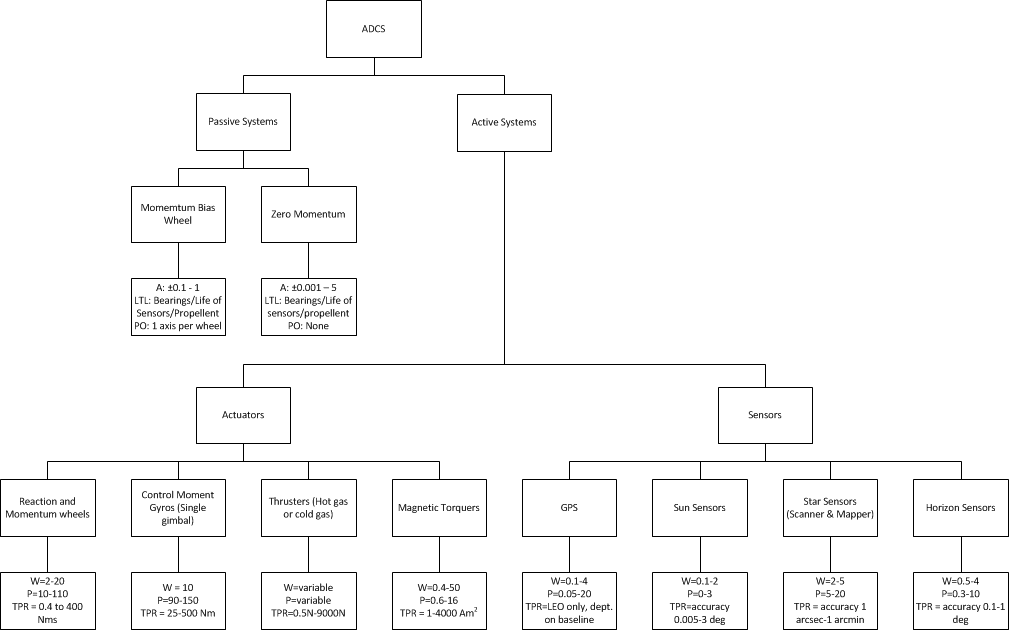
\includegraphics[width=1.0\textwidth, angle=90]{chapters/img/prunedADCStree.png}
\label{fig:pruneADCS}
\caption{Pruned design option tree for the \acs{ADCS}}
\end{figure}

%%%%%%%%%%%%%%%%%%%%%%%%%%%%%%%%%%%%%%%%%%%%%%%%%%%%%%%%%%%%%%%%%%%%%%%%%%%%%%%%%%%%
\subsection{\acl{ADS}}
\label{ss:ads}
The \ac{ADS} consists for a collection of sensors to determine the roll, pitch and yaw angles and rates of the satellites. The design options left after the pruning in section \ref{pruneADCS} are \ac{GPS}, Sun sensors, Star trackers and horizon sensors. 

\ac{GPS} uses one receiver and multiple antennas. By measuring the relative positions of the different antennas the attitude of the satellite can be calculated. Most modern \ac{LEO} satellites are already carrying a \ac{GPS} receiver, but a long baseline between antennas is needed for a high accuracy. 

Sun sensors use the angle towards the Sun for making their attitude measurements. The technology behind Sun sensors has been around for a long time and several micro Sun sensors are available on the market. The \ac{FOV} of a typical Sun sensor is about 120${}^{\circ}$.

Star trackers look at a portion of the sky and use familiar stars to determine the attitude of the satellites. This system can work autonomously, but the optics required are usually quite bulky.

Horizon sensors use the limb of the Earth, i.e. the transition of the solid Earth to cold space, to determine the attitude of the satellite. The system only works on the roll and pitch axes.

Another option is to use a complete \ac{COTS} \ac{ADCS} system like the one from Maryland Aerospace Inc. \cite{maryland}. Their IMI-100 ADACS contains everything needed for complete \ac{ADCS} with an accuracy of 1${}^\circ$. For attitude determination it uses 3 magnetometers, by adding additional sensors e.g. a ring laser gyro and a miniaturised star sensor the accuracy can reach 1-3 arcsec \cite{imi100}.

\subsubsection{Trade method}
The trade-off is made by comparing three concepts for attitude determination. The first concept uses the Maryland Aerospace IMI-100, the second concept uses Sun sensors by day and a star tracker by night, the third concept uses \ac{GPS} for attitude determination (see figure \ref{fig:adsconcepts} on page \pageref{fig:adsconcepts}. Scores are awarded to the performance on a number of criteria. The best weighed overall score wins the trade-off.

\begin{figure}[h]
\centering
$\begin{array}{c c c}
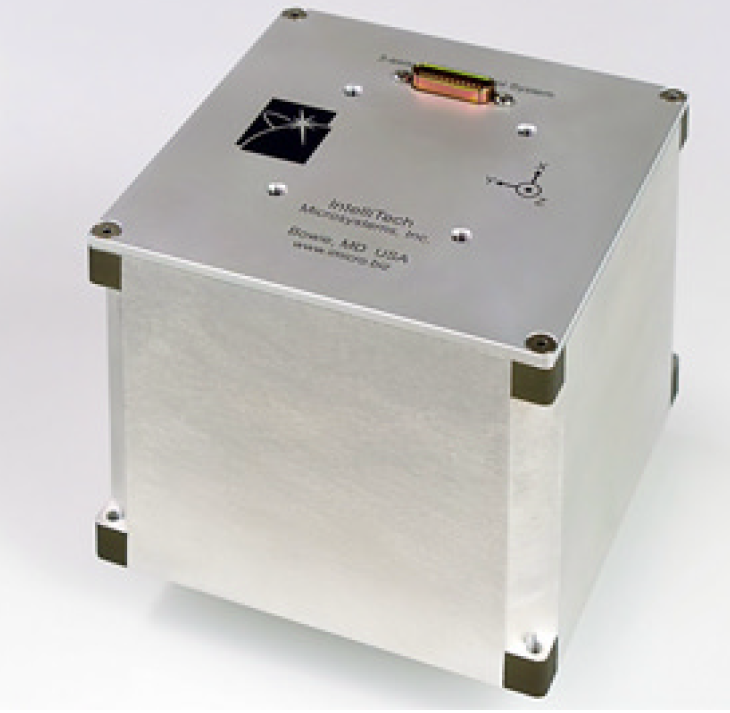
\includegraphics[height = 120px]{chapters/img/imi100attitude.png}    
& 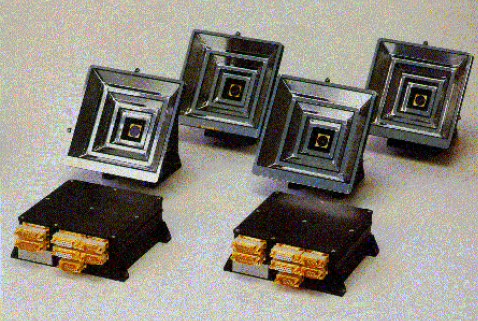
\includegraphics[height = 120px]{chapters/img/sunsensorattitude.png} 
& 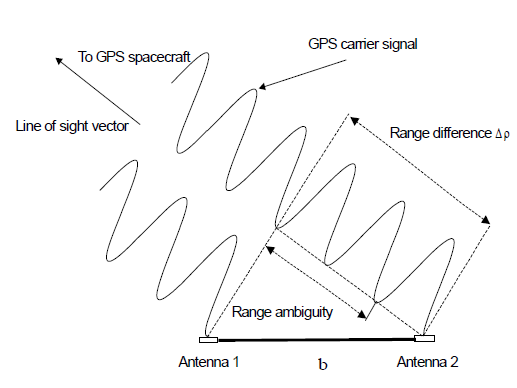
\includegraphics[height = 120px]{chapters/img/gpsattitude.png} 
\end{array}$
\caption[\acs{ADS} design concepts]{The three concepts for the design of the \ac{ADS}. From left to right: Concept 1 uses the IMI-100 system from Maryland Inc. \cite{imi100}, concept 2 uses Sun sensors and star trackers \cite{chu21}, concept 3 uses \ac{GPS} for attitude determination \cite{chu21}}
\label{fig:adsconcepts}
\end{figure}

\subsubsection{Trade criteria}
The concepts for \ac{ADS} are traded in terms of attitude determination accuracy, purchasing price, power required, size and the amount of additional development required for implementing the concept. 
\subsubsection{Weight factors}
The accuracy of the \ac{ADS} is the main driver for the choice of the system so it is given a weight factor of 9. Because the volume and power for satellites are limited they are also important with a given weight factor of 7. Although the total cost of the system is relevant, if a better performance can be achieved at a higher cost that can be acceptable, wherefore it is given a weight factor 3. If a lot of work still is required to implement the system in the satellite the mission can be delayed, development gets a weight factor of 5.
\subsubsection{Trade-off}
The results of the trade-off can be found in table \ref{tab:adstradeoff} on page \pageref{tab:adstradeoff}. 
The attitude determination accuracy of concept 1 and concept 3 are both around $1^\circ$ for micro satellites, the performance of concept 2 is much better with an estimated accuracy of $0.01^\circ$. 
In the \ac{ISIS}' webshop \cite{cubesatshop} concept 1 costs about EUR 45000, the development costs of concept 2 are estimated to be about EUR 15000, a space qualified \ac{GPS} receiver will cost about EUR 25000 \cite{spacequest}.
The first concept will use about 1.5 W on attitude determination, concept 2 uses a power of about 2 W, a \ac{GPS} receiver takes about 1 W.
The size of the IMI-100 is 100x100x79 mm, the Sun sensors can be as small as 30x30x14.5 mm \cite{tnoweb} and \ac{ISIS} is currently developing a star sensor with a size of 50x50x100 mm, a space qualified \ac{GPS} receiver is about 100x70x25 mm. 
The IMI-100 system is completely developed and can just be build in, for a system with Sun sensors and a star tracker still some design needs to be done in for example locations on the satellite, for a \ac{GPS} system the antenna positions need to be chosen for optimal accuracy.

\begin{table} [h]
\centering
\begin{tabular}{p{3cm} | c | c c c}
\textbf{Criteria} & \textbf{Weight Factor} & \textbf{Concept 1} & \textbf{Concept 2} & \textbf{Concept 3} \\ \hline \hline
Accuracy    & 9 & 4 & 8 & 4\\
Size        & 7 & 2 & 6 & 4\\
Power       & 7 & 6 & 5 & 7\\
Price       & 3 & 3 & 5 & 4\\
Development & 5 & 8 & 4 & 5\\ \hline
Weighted total    &    & 141 & 184 & 150
\end{tabular} 
\caption[Trade-off attitude determination]{Trade-off graph for the attitude determination system. The weight factor signifies the importance of the criterion. Grades are given on a scale of 1 to 10, 1 being the worst, 10 the best}
\label{tab:adstradeoff}
\end{table}

After the trade-off the best solution for the \ac{ADS} is to use Sun sensors and a star tracker. Although the most design work is needed, it is able to give the best accuracy for the lowest price.  

%%%%%%%%%%%%%%%%%%%%%%%%%%%%%%%%%%%%%%%%%%%%%%%%%%%%%%%%%%%%%%%%%%%%%%%%%%%%%%%%%%%%
\subsection{\ac{ACS}}
\label{ss:acs}
The satellites in the constellation all need to point accurately to the Earth, a passive \ac{ACS} will therefore not be sufficient for the control of the attitude of the satellites. For active attitude control actuators are needed. After the pruning, four options remain for the attitude control. Reaction and momentum wheels, \acp{CMG}, Thusters and Magnetic torquers.

Reaction wheels are basically torque rotors with a high-inertia wheel attached to it; they can provide single axis control to a spacecraft. Momentum wheels are reaction wheels with a nominal spin rate, adding gyroscopic stiffness to two axis of the spacecraft. Changing the spin rate gives control over the third axis.
\acp{CMG} consist of a wheel with a constant rotation speed and one or two gimbals to rotate the wheel, determining the direction of the momentum. This way very accurate attitude manoeuvres can be made, but complex control algorithms are needed. Usually the weight and cost of \acp{CMG} are quite high.
Thusters expel mass to induce velocity or a momentum to the satellite. The velocity can be used for keeping the orbit and will be discussed in section \ref{ss:ocs}. To be able to induce a momentum to a satellite multiple thrusters with an offset to the center of mass of the satellite. Thrusters are split up into hot gas types, which require a chemical reaction of the propellent, and cold gas types that rely on latent heat and phase change in the propellent. The power which can be generated by thrusters is high, but the fuel required will limit the lifetime of the satellite.
Magnetic torquers are magnetic coils or electromagnets generating dipole moments on the satellite. They can be used for both manoevering and desaturation of e.g. reaction wheels. Because they rely on the magnetic field of the Earth they are less useful in higher orbits.

The IMI-100 ADACS contains three miniature reaction wheels and three magnetic coils for desaturating the wheels. For a 2 kg, 2U cubesat it can provide a slew rate of $8.4^\circ/s$ \cite{imi100}.

\subsubsection{Trade method}
In the trade-off three concepts for attitude control are compared to each other on a number of criteria. The first concept is using thrusters for attitude control, the second option is using reaction wheels with magneto torquers for desaturation, the third option is using Maryland Aerospace's IMI-100. The concept with the highest weighted score wins the trade-off. The options are shown in figure \ref{fig:acsconcepts} on page \pageref{fig:acsconcepts}.

\begin{figure}[h]
\centering
$\begin{array}{c c c}
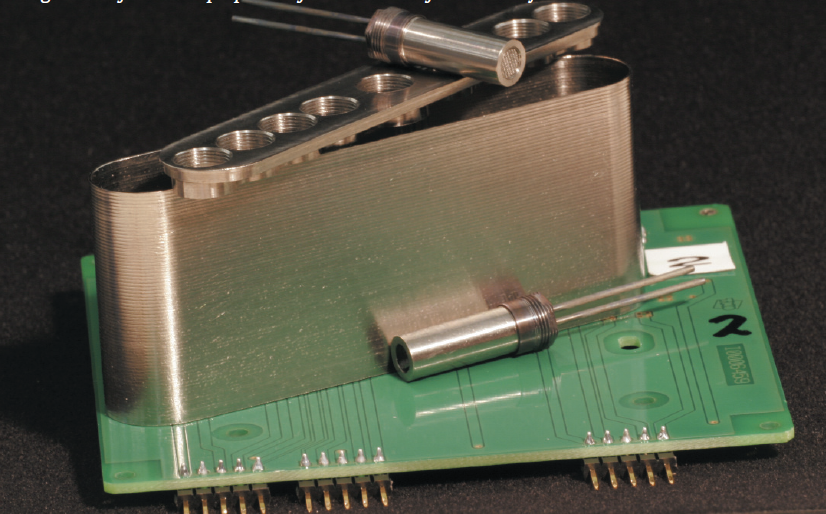
\includegraphics[height = 120px]{chapters/img/thrusterattitude.png} 
& 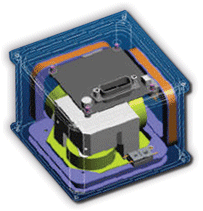
\includegraphics[height = 120px]{chapters/img/reactionattitude.png} 
& 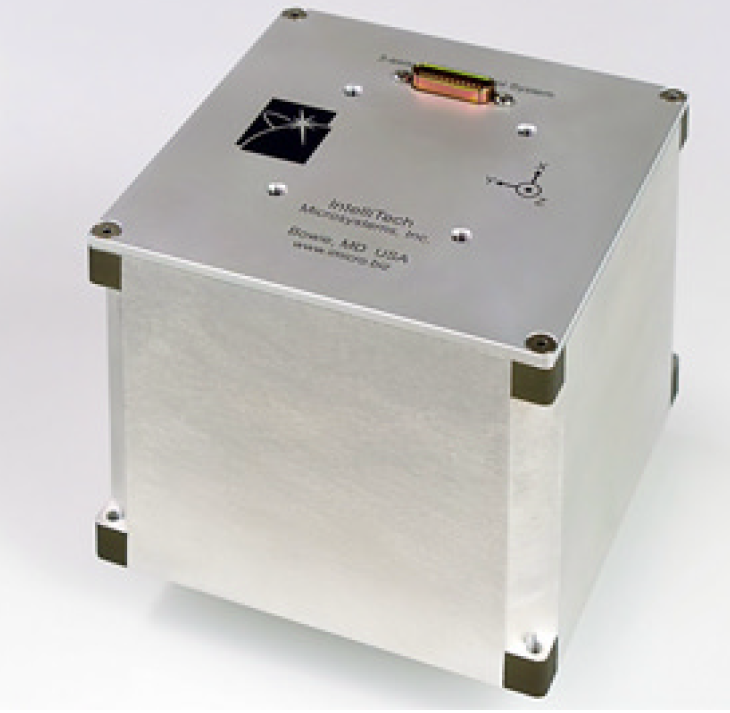
\includegraphics[height = 120px]{chapters/img/imi100attitude.png} 
\end{array}$
\caption[\acs{ADS} design concepts]{The three concepts for the design of the \ac{ADS}. From left to right: Concept 1 uses thrusters \cite{tnoweb}, Concept 2 uses reaction wheels and magneto torquers \cite{cubesatshop}, Concept 3 uses IMI-100 system from Maryland Inc. \cite{imi100}.}
\label{fig:acsconcepts}
\end{figure}

%, bb =0 0 826px 514px          , bb=0 0 203px 211px            , bb=0 0 730px 713px

\subsubsection{Trade criteria}
The concepts for \ac{ACS} are traded in terms of the rate the concepts are able to adjust the attitude, attitude control accuracy, purchasing price, power required, size and the amount of additional development required for implementing the concept. 
\subsubsection{Weight factors}
A high rate in which the satellite can be controlled is convenient, but not driving, weight factor 5. Since attitude control will be used for the pointing of the instrument the accuracy is very important for the choice so it is given a weight factor of 8. Because the volume and power for satellites are limited they are also important with a given weight factor of 7. Although the total cost of the system is relevant, if a better performance can be achieved at a higher cost can be acceptable, weight factor 3. If a lot of work still is required to implement the system in the satellite the mission can be delayed, development gets a weight factor of 5.
\subsubsection{Trade-off}
The results of the trade-off can be found in table \ref{tab:acstradeoff} on page \pageref{tab:acstradeoff}.
Thrusters are able to make attitude adjustments with a high rate, both concept 2 and concept 3 use reaction wheels for attitude adjustments, so they will have comparable performance.
Attitude adjustments done by thrusters are really coarse, so they have a low accuracy. With a custom designed system the accuracy of concept 2 the performance will be better than a \ac{COTS} system.
For the use of thrusters also other components are required like e.g. fuel tanks, fuel lines and pumps. Reaction wheels and magneto torquers all take up space in the satellite, but can be made relatively small The IMI-100 system is encased in a separate box, so it will take more room.
For its power the thruster system needs fuel, which all has to be taken along for the entire mission. The reaction wheels in concept 2 and 3 require only power when the motors are running, as do the magneto torquers.
Combined with the fuel, tanks and other extra material the thruster system needs to bring it will be a very expensive option. Especially for the small kind of satellites being considered for the mission. Not many micro propulsion systems are yet on the market. Developing the system with reaction wheels can be a much cheaper option. Buying the system as \ac{COTS} will save working costs, but in the end be a little more expensive than a in house development.
Thruster systems for small satellites are rare, so a lot of development is still required. Some research has already been done on an active \ac{ACS} for the student satellite Delfi-n3Xt \cite{delfispace}, this research can be extended for the Laser Swarm mission. The IMI-100 system is already build and just has to be integrated. 

\begin{table} [h]
\centering
\begin{tabular}{p{3cm} | c | c c c}
\textbf{Criteria} & \textbf{Weight Factor} & \textbf{Concept 1} & \textbf{Concept 2} & \textbf{Concept 3} \\ \hline \hline
Rate 	    & 5 & 8 & 6 & 6 \\
Accuracy    & 8 & 4 & 8 & 7 \\
Size        & 7 & 2 & 6 & 5 \\
Power       & 7 & 3 & 6 & 6 \\
Price       & 3 & 2 & 8 & 7 \\
Development & 5 & 4 & 6 & 8 \\ \hline
Weighted total    &    & 133 & 232 & 224
\end{tabular} 
\caption[Trade-off attitude control]{Trade-off graph for the attitude control system. The weight factor signifies the importance of the criterion. Grades are given on a scale of 1 to 10, 1 being the worst, 10 the best}
\label{tab:acstradeoff}
\end{table}

After the trade-off the best solution for the \ac{ACS} is to use reaction wheels and magneto torquers. Although the scores are close to concept 3, the more dedicated design improves the performance of the \ac{COTS} system.

%%%%%%%%%%%%%%%%%%%%%%%%%%%%%%%%%%%%%%%%%%%%%%%%%%%%%%%%%%%%%%%%%%%%%%%%%%%%%%%%%%%%
\subsection{\ac{ODS}}
\label{ss:ods}
The determination of the orbit will be discussed in section \ref{TOcommTA}.

%%%%%%%%%%%%%%%%%%%%%%%%%%%%%%%%%%%%%%%%%%%%%%%%%%%%%%%%%%%%%%%%%%%%%%%%%%%%%%%%%%%%
\subsection{\ac{OCS}}
\label{ss:ocs}

The \ac{OCS} needs to counter the atmospheric drag forces with the $\Delta V$ calculated in section \ref{mtrOrbAltitude}. The $\Delta V$ a propulsion system can produce is quantified by Tsiolkovsky's rocket equation

\begin{equation}
\Delta V = g I_{sp} \ln{\left(\frac{m_0}{m_0-m_p}\right)}\equiv g I_{sp} \ln{\left(\frac{m_0}{m_f}\right)} \equiv g I_{sp} \ln{\left(R\right)}
\label{eqn:tsiolkovsky}
\end{equation}

where $g$ is the Earth's gravity constant, $I_{sp}$ is the specific impulse of the engine, $m_0$ is the starting mass, $m_p$ is the mass of the fuel used, $m_f = m_0-m_p$ and the mass ratio $R$ is  ${m_0}/\left({m_0-m_p}\right)$. From this the ratio of fuel to the total mass can be derived to be

\begin{equation}
\frac{m_p}{m_0} = 1-e^{-\left(\Delta V/I_{sp}g\right)}
\label{eqn:fuelratio}
\end{equation}

Depending on the altitude of the satellite orbit a thruster for attitude keeping can be selected in a later stage of the design.